%%%%%%%%%%%%%%%%%%%%%%%%%%%%%%%%%%%%%%%%%%%%%%%%%%%%%%%%%%%%%%%%%%%%%%%%%%%
\begin{figure*}[tbp!]
%\centering
\hspace{-6mm}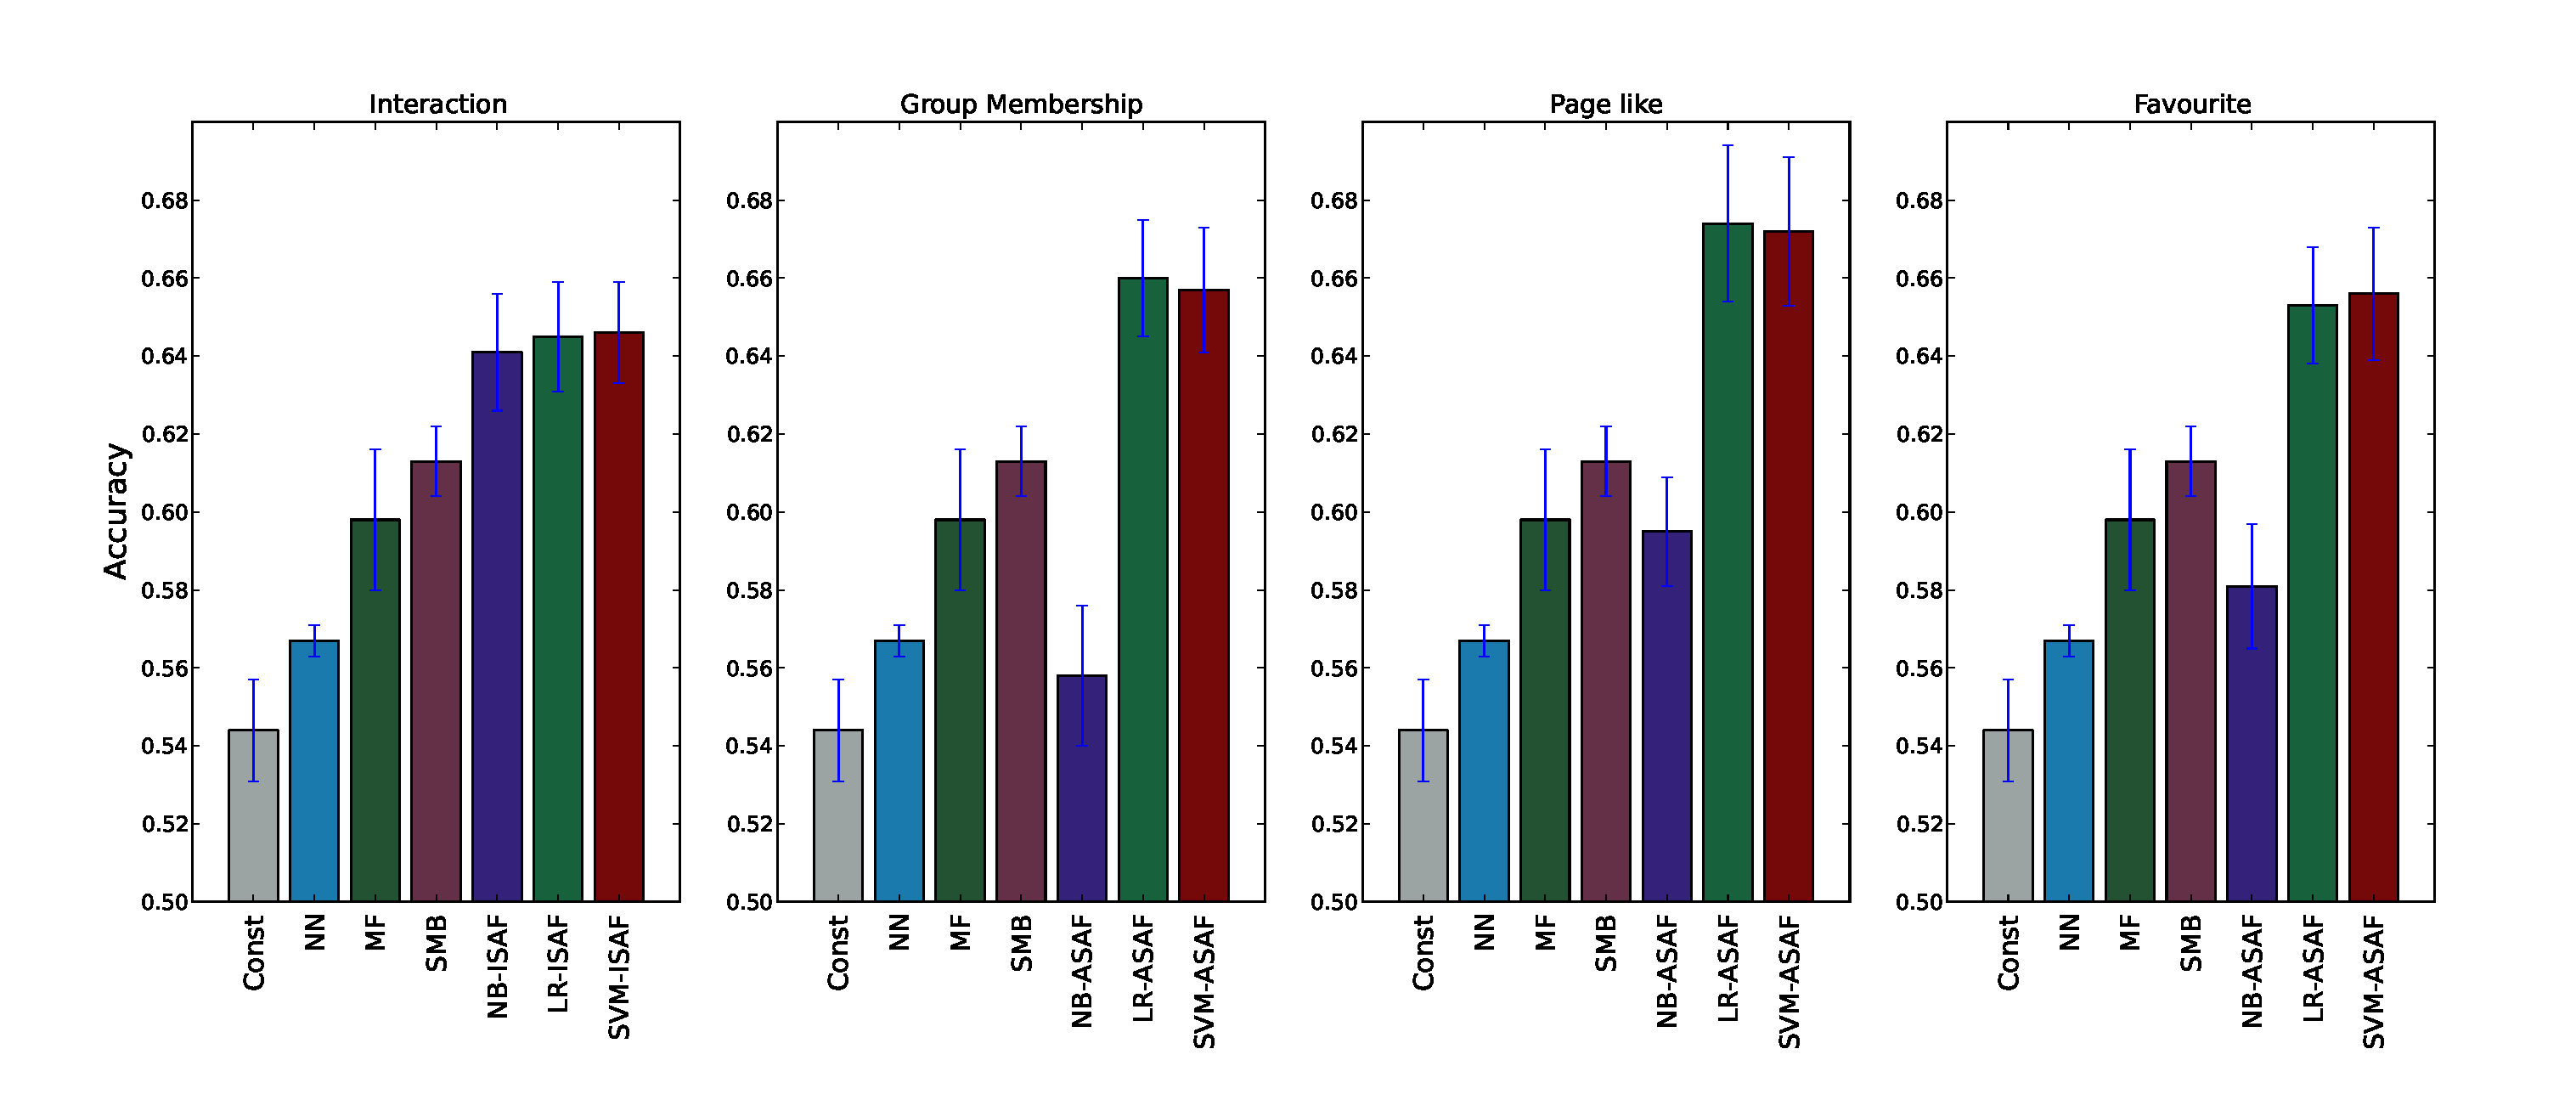
\includegraphics[width=180mm,height=60mm]{data/plots/accuracy/accuracyLargeNew.eps}
\caption{  Comparision of the standard collaborative filtering algorithms with proposed SAF based models.  SAF based models significantly outperforms standard collaborative filtering and social recommender systems, by up to 6 \% in accuracy. }
\label{Fig1}
\end{figure*}
%%%%%%%%%%%%%%%%%%%%%%%%%%%%%%%%%%%%%%%%%%%%%%%%%%%%%%%%%%%%%%%%%%%%%%%%%%%

In this section, we compare novel SAF-based model trained on naive Bayes(NB), 
logistic regression (LR) and support vector machine (SVM) to the variety of
(social) collaborative filtering baselines. For baselines, we examine the most 
likely class constant predictor (Const), and state-of-the-art collaborative 
filtering algorithms: Nearest Neighbor (NN)~\cite{bellkor}, Matrix Factorization (MF)~\cite{pmf} 
and Social MatchBox (SMB)~\cite{Noel2012NOF} -- an extension of matrix
factorization that encourages more homophily for pairs of users with
more interactions. To make a distinction between Interaction and Activity based SAF, 
we add a suffix ISAF and ASAF respectively to NB, LR and SVM as shown in Fig~\ref{Fig1}. We train model using
10-fold cross validation and the error bars corresponds to 95\% confindence interval.

Fig~\ref{Fig1} compares the accuracies of the baseline methods 
with the SAF based models for a range of interaction and activity (group,
page, favourite) SAGs.  In all of our experiments SAF variants
performed significantly better than state-of-the-art in social
collaborative filtering (SCF) as represented by Social
Matchbox~\cite{Noel2012NOF} and other baselines except for na\"{i}ve Bayes, 
we conjecture this is due to the correlations between SAGs that cause na\"{i}ve
Bayes to over- or under-estimate the true probability of likes. Furthermore, Fig~\ref{Fig1} 
shows that the page like yields the most accurate predictor among the interaction and activities SAGs.
This may indicate the fact that page likes are relatively more indicative of user preferences.

%Fig \ref{Fig1} shows that the page likes were the most predictive among
%the interaction and activities SAGs. Furthermore, these results may indicate
%that there is more social affinity between users having same page likes
%than other activities. Returning to our conjecture that data 
%sparsity can hurt SAF, we note from Table~\ref{tab:interests} that page 
%likes are more prevalent than groups and favourites. 

%In general we note in Fig~\ref{Fig1} that activities appear to be
%more predictive than interactions, but we believe the reasons for this
%are quite simple: Interaction SAGs can only evaluate the friends of
%user $u$ whereas Activity SAGs are able to look at all users,
%independent of $u$'s friends.
%Hence, given the general sparsity of ``likes'' data in Facebook, 
%Activity SAGs appear to draw on a much larger group of SAGs
%with much more activity.



%Among activities, Fig \ref{Fig1} shows that activities are more
%predictive than interactions. Among the activities, page likes are the
%most predictive followed by group membership and favourites.
%Returning to our conjecture that data sparsity can hurt SAF, we note
%from Table~\ref{tab:interests} that page likes are more prevalent than
%groups and favourites.  Moreover, these results may indicate that
%there is more social affinity between co-members of inherently social
%activities like groups and pages than between users who simply have
%favourites in common.

We note that the key difference of SAF vs. SCF is
that SAF exploits the predictiveness of fine-grained interactions, whereas most SCF
approaches~\cite{Noel2012NOF,lla,socinf,sr,rrmf,ste} collapse a diverse set
 of interactions into aggregate statistics such as the number of interactions 
between user $u_1$ and user $u_2$, regardless of different modality, action and direction.
%Clearly there is a great deal of benefit deriving from the fine-grained 
%interactions indicating why without modeling any latent space and using 
%a simple linear classifier, SAF can outperform SCF methods based on matrix
%factorization approaches that attempt to learn latent user and item
%features. 
On a final note, we remark that SAF is more robust to cold start 
problem: this is because SAF learns from the SAGs which are derived from 
inherently available user's social network information (interactions and activities).

%On two final notes, we remark that SAF yields a computational and
%optimization advantage over SCF in that it is straightforward and
%efficient to find a globally optimal classifier with respect to certain training
%criteria (e.g., optimising log loss in logistic regression or hinge
%loss in SVMs) unlike SCF approaches that generally rely on
%computationally expensive matrix factorization techniques that lack
%optimality guarantees.  Further, we also note quite surprisingly that
%SAF inherently scales to a large number of users and generalizes to
%completely new users without suffering from the cold-start problem:
%this is simply because nothing SAF learns is user dependent, it learns
%to weight SAGs independent of any particular user.

Given the benefits of SAF, we now proceed in the
next section to analyse the two primary types of SAG features
(interactions and activities) to better understand characteristics of
both informative and uninformative SAGs in each context and the social
phenomena that may be responsible for these characteristics.